\documentclass{beamer}
\usetheme{AnnArbor}
\usecolortheme{crane}

\title{Image Inpainting with Deep Learning}
\author{Ian Li}
\institute{Harvey Mudd College}
\begin{document}
\frame{\titlepage}
\begin{frame}
	\tableofcontents
\end{frame}

\section{Introduction}
\begin{frame}
	\frametitle{Overview of Image Inpainting}
	\begin{itemize}
		\item Definition: Filling in missing or damaged areas of digital images.
		\item Purpose: 
		\begin{itemize}
			\item Enhance photo quality
			\item restore historical images
			\item edit content
		\end{itemize}
	\end{itemize}
	\begin{center}
		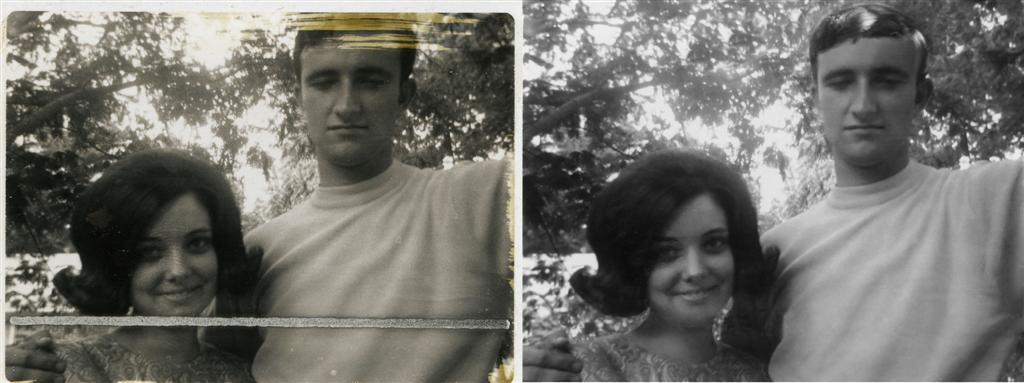
\includegraphics[scale=4]{restoration.jpeg}
	\end{center}
\end{frame}

\begin{frame}
	\frametitle{How Does Image Inpainting Work (Traditionally)?}
	\begin{itemize}
		\item Patch-based methods: patches from the surrounding areas are used to fill in gaps
		
		\begin{center}
			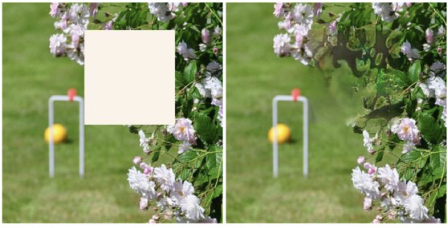
\includegraphics[scale=0.8]{patch.png}
		\end{center}
		
		\item Limitations:
		\begin{itemize}
			\item  Surrounding regions might not have suitable information
			\item Missing regions require the inpainting system to infer properties of the would-be-present objects
		\end{itemize}
		\item With a Deep Learning approach, we can better capture spatial contexts in  images
	\end{itemize}
\end{frame}

\section{Data}
\begin{frame}
	\frametitle{CIFAR10 Dataset}
	\begin{itemize}
		\item A widely used dataset in ML, containing 60,000 32x32 color images across 10 classes
		\item Provides a benchmark for comparing different methods and tracking progress in the field
	\end{itemize}
	\begin{center}
		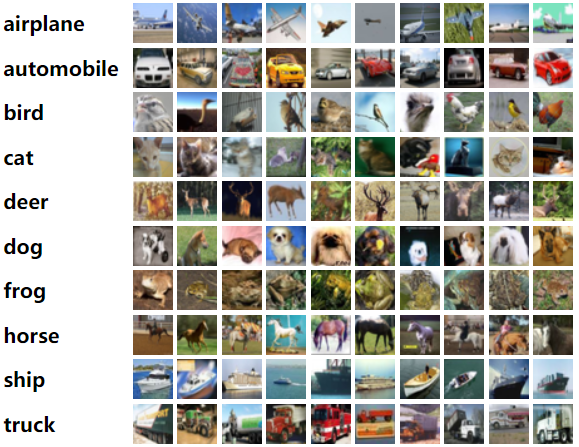
\includegraphics[scale=0.3]{cifar10.png}
	\end{center}
\end{frame}

\begin{frame}
	\frametitle{Data Preparation}
	\begin{itemize}
		\item Inpainting is a process of reconstructing lost or deteriorated parts of images
		\item Add artificial deterioration to our images through masking
		\begin{itemize}
			\item Drew lines of random length and thickness using OpenCV
		\end{itemize}
	\end{itemize}
	\begin{center}
		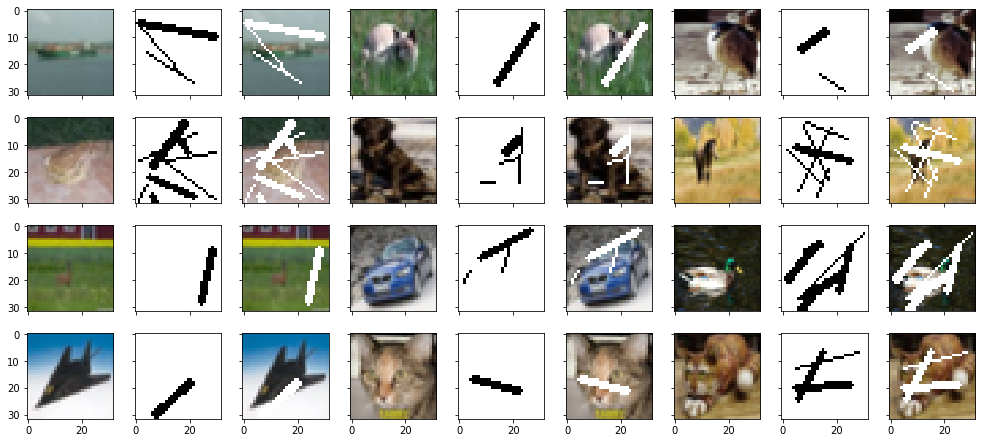
\includegraphics[scale=0.3]{masks.png}
	\end{center}
\end{frame}
\section{Methods}
\begin{frame}
	\frametitle{Convolutional Autoencoders}
	\begin{itemize}
		\item Autoencoders: a type of neural network that can be used to learn a compressed representation of a dataset
		\item Encoder: maps the input data to a lower-dimensional representation
		\item Decoder: maps the lower-dimensional representation back to the original dimensionality
	\end{itemize}
	\begin{center}
		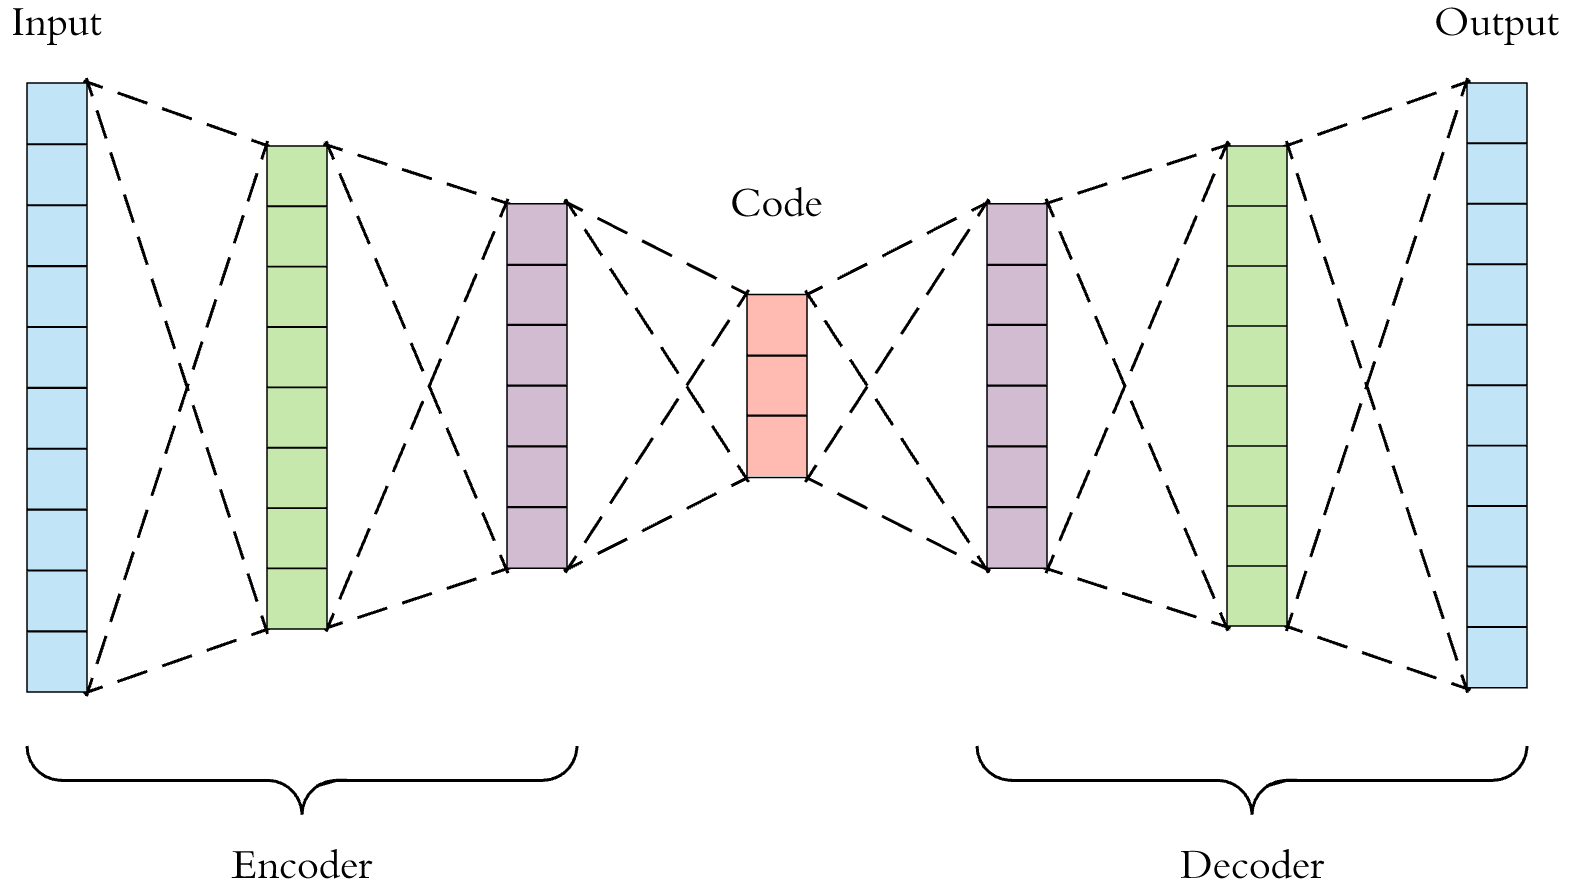
\includegraphics[scale=0.1]{autoencoder.png}
	\end{center}
	\begin{itemize}
		\item Convolutions: learn hierarchical representations of data including shapes, edges, etc.
	\end{itemize}
\end{frame}

\begin{frame}
	\frametitle{Partial Convolutions}
	\begin{itemize}
		\item In traditional convolutional layers, missing pixels are also used for convolution, resulting in poor image quality.
		\item We wish to only use valid pixels to learn representations 
		\begin{center}
		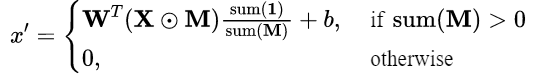
\includegraphics[scale=0.5]{partial1.png}
		\end{center}
		\item After each partial convolution operation, we then update the mask
		\begin{center}
			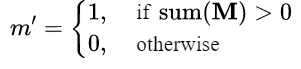
\includegraphics[scale=0.5]{partial2.png}
		\end{center}
	\end{itemize}
	
\end{frame}

\begin{frame}
	\frametitle{Dice Coefficient}
	\begin{center}
		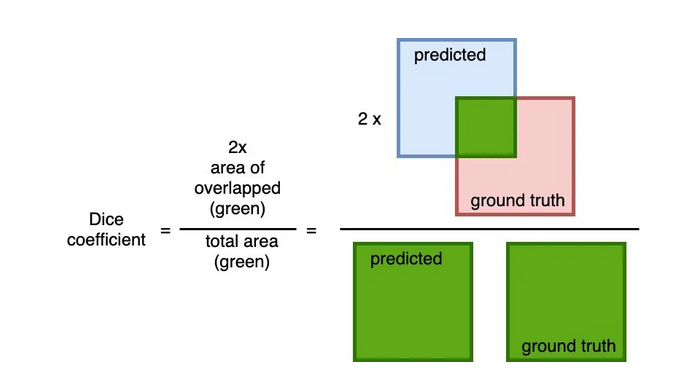
\includegraphics[scale=0.4]{dice.png}
	\end{center}
	\begin{itemize}
		\item Measures the accuracies of our predictions!
	\end{itemize}
\end{frame}


\section{results}
\begin{frame}
	\frametitle{Convolutional Autoencoder Results}
	\begin{center}
		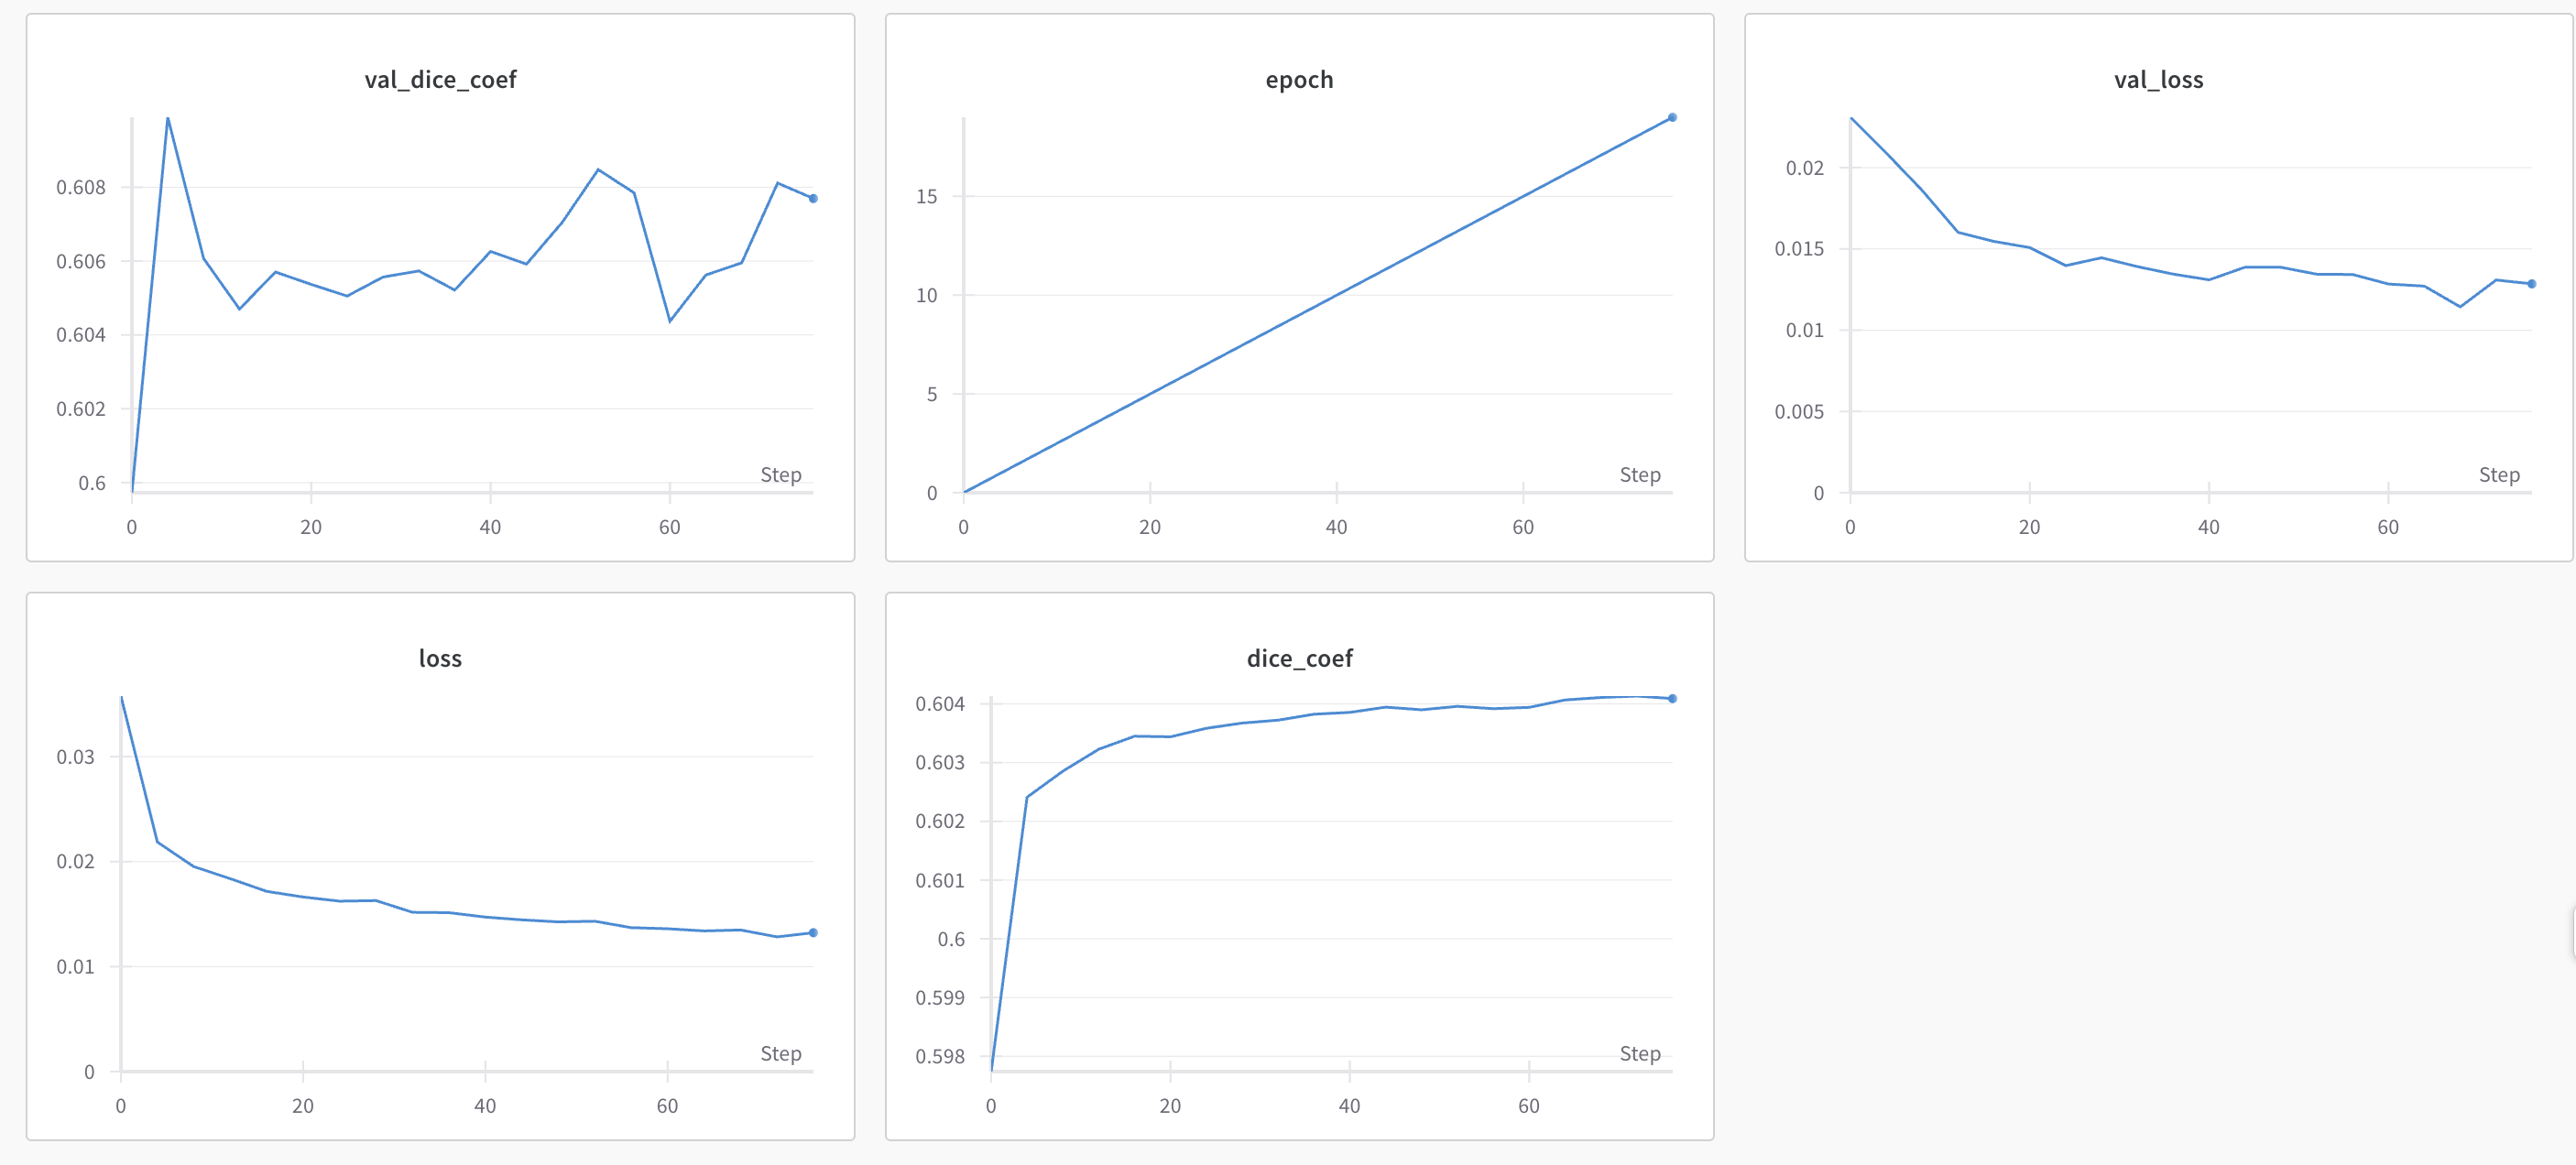
\includegraphics[scale=0.25]{result1.png}
	\end{center}
\end{frame}

\begin{frame}
	\frametitle{Partial Conv Autoencoder Results}
	\begin{center}
		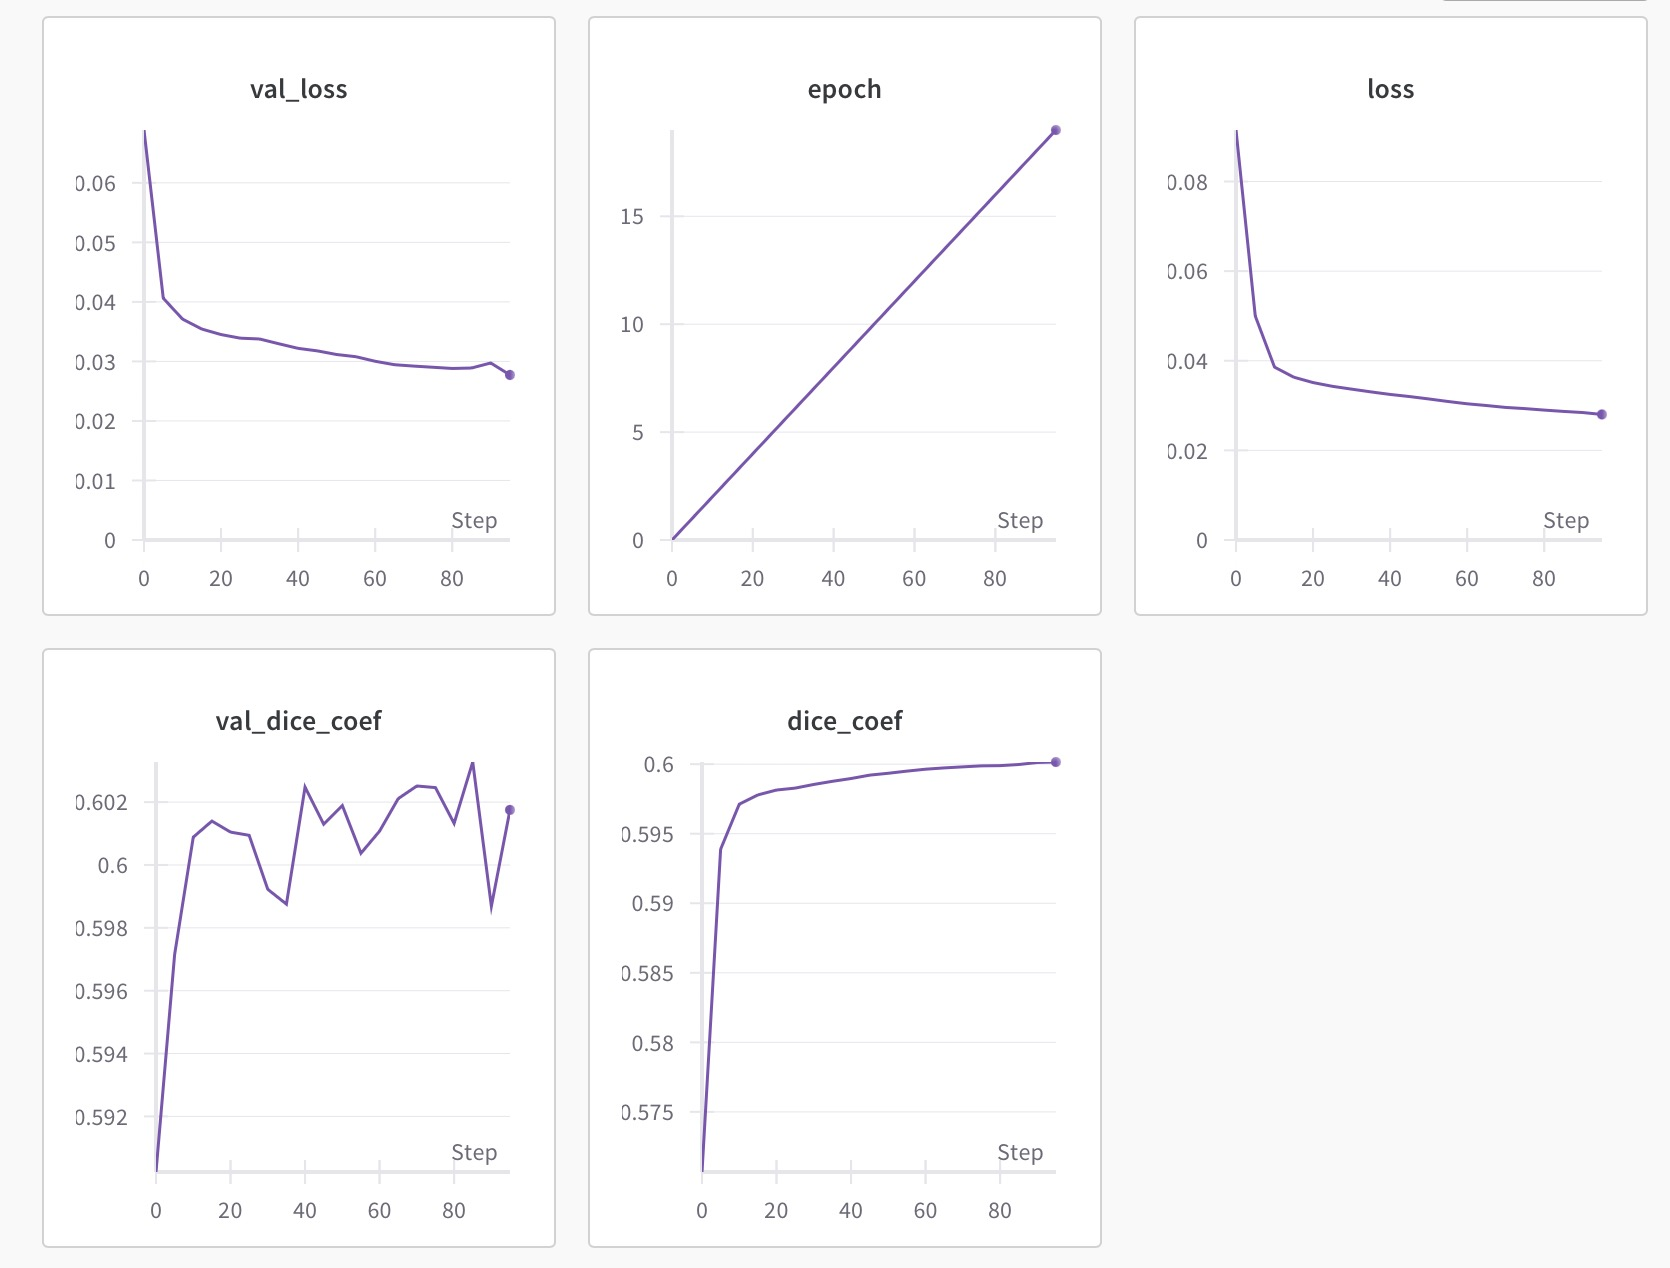
\includegraphics[scale=0.3]{results2.jpg}
	\end{center}
\end{frame}

\section{Next Steps}
\section{results}
\begin{frame}
	\frametitle{Next Steps}
	\begin{itemize}
		\item Test both methods on higher resolution datasets
		\item Image inpainting with stable diffusion
		\item Tractibility of Diffusion Models
	\end{itemize}
\end{frame}

\end{document}
